\section{Modelling Previous Design}\label{sec:old-design-method}
As mentioned earlier, microgravity is incredibly costly to achieve experimentally, so a numerical investigation of the old design was conducted using Ansys Fluent. The simulation was set up and then ran once with gravity and once without, comparing the distribution of powder within the tank and the mass flow rate. An axisymmetric, fine mesh simulation was first conducted as it would have maintained the same quantities as a 3D simulation while running much faster. This proved numerically unstable, therefore, a 2D simulation with a much coarser mesh of 1mm square cells was conducted, seen in \autoref{fig:old-design-sim}.
\begin{figure}[htbp]
    \centering

    \begin{minipage}{0.3\textwidth}
        \centering
        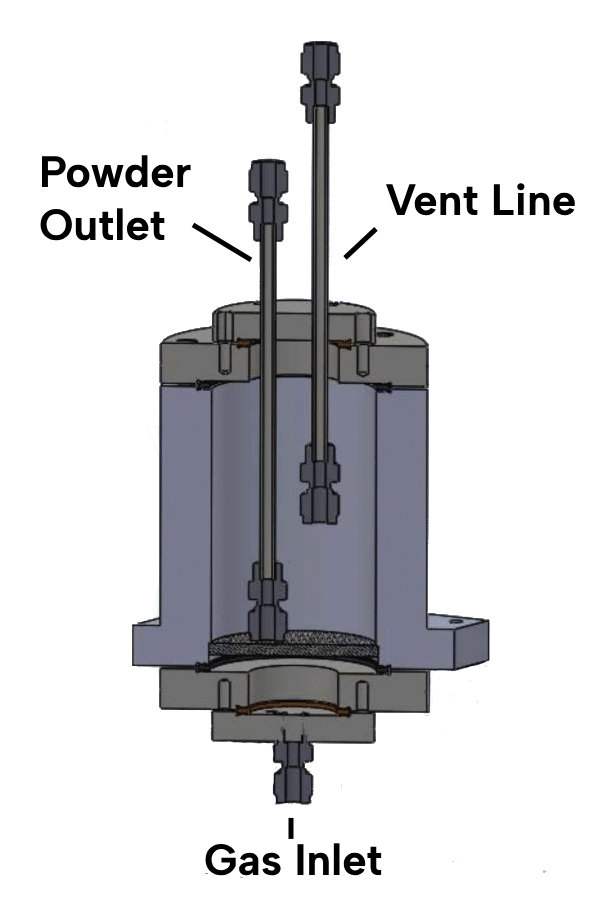
\includegraphics[width=\textwidth]{../report_assets/COSMOS_DIAGRAM_2x3.png}
        \caption*{(a) Previous Design}
    \end{minipage}
    \hfill
    \begin{minipage}{0.3\textwidth}
        \centering
        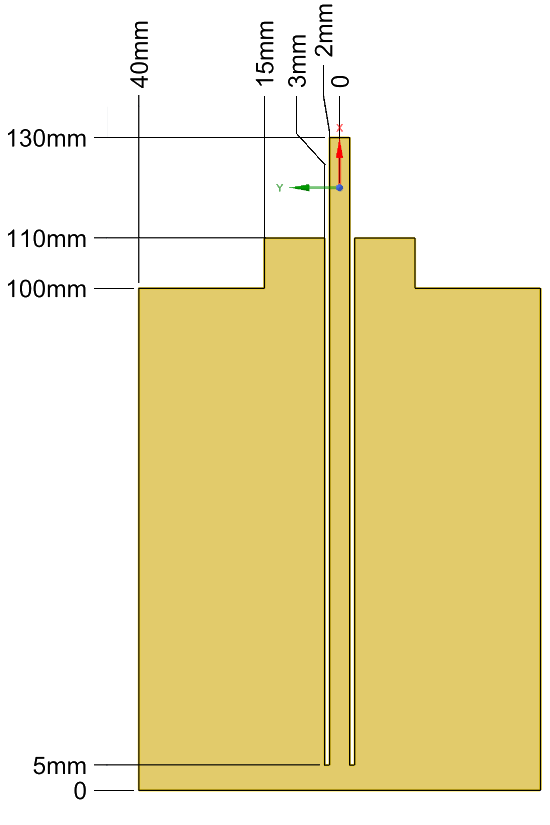
\includegraphics[width=\textwidth]{../report_assets/geom_old.png}
        \caption*{(b) Simplified Geometry}\label{fig:idkyet9}
    \end{minipage}
    \hfill
    \begin{minipage}{0.3\textwidth}
        \centering
        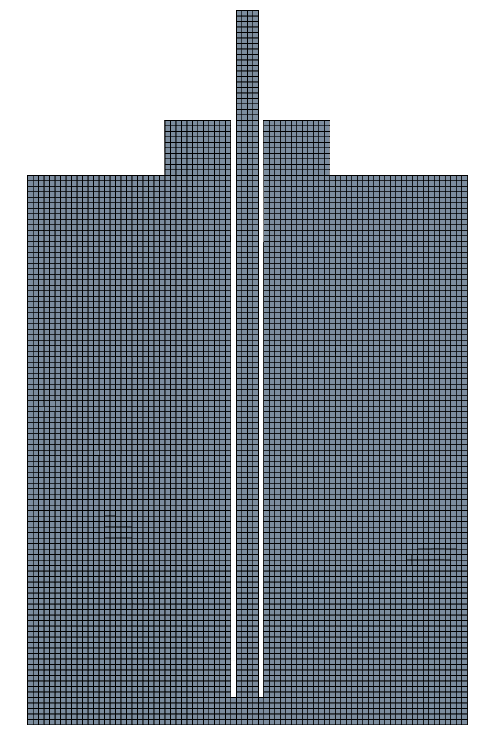
\includegraphics[width=\textwidth]{../report_assets/mesh_old.png}
        \caption*{(c) Mesh Used for Sim}\label{fig:idkyet10}
    \end{minipage}
    
\end{figure}\label{fig:old-design-sim}
While the 2D nature of the simulation means that none of the quantities are representative of the real 3D physics, the key flow characteristics of interest are still expected to remain. 
A simplified geometry, seen in \autoref{fig:old-design-sim} (b), was used as it speads up computational time while still preserving the physics of interest. The vent line pipe was omitted and the outlet pipe was moved to the center, neither of these are expected to impact on the behaviour being investigated. The bottom of the tank held the wire mesh on which the powder sat. The bottom of the surface represents this mesh, acting as the velocity inlet of the simulation at 0.1m/s. To simulate the two phases, a eulerian-eulerian model was used with a gidaspow drag model as this has been shown to best represent fluidising beds~\cite{C6RA28615A}. The powder was modelled as TI6AL4V as this was what was used in the prior testing. Typical titanium allow powder used in SLS printing has a particle size distribution between 15 and 53um and a density between 2.04 and 2.34g/cm3~\cite{ma17040952}. It is assumed this is similar to the powder used in CSAM and therefore a 40um particle size and 2200kg/m3 density was used. The gas was modelled as air at standard operating conditions.

\section{Choosing New Feed System Architecture}\label{sec:system_architecture}
As discussed in \autoref{sec:prev-design-analysis}, a new design was desirable and research into current powder feed technology was conducted. While every effort was made to review analogous systems reported in the literature, time constraints mean that the author cannot rule out overlooking relevant works. The only research found on powder-based AM experiments conducted in microgravity originate from the Fraunhofer Institute for Transportation and Automation Technology, but those reports offer scant detail on the powder-feed mechanism employed~\cite{OVERMEYER2025}. Accordingly, five common terrestrial powder-dispensing methods were examined, and the modifications required to adapt each for use in a space environment were evaluated. Basic schematics of these methods are presented in \autoref{fig:powder-dispensing-methods} and the full analysis can be found in \autoref{appendix:feed-architecture-analysis}. 
\begin{figure}[htbp]
    \centering

    % First row: 3 images
    \begin{minipage}{0.3\textwidth}
        \centering
        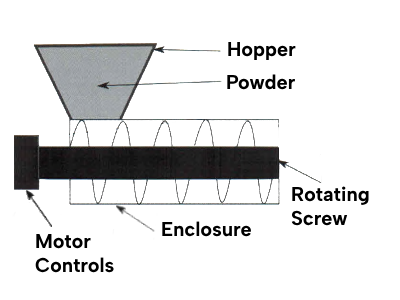
\includegraphics[width=\textwidth]{../report_assets/screw_feed_polished.png}
        \caption*{(a) Screw Fed Design~\cite{Bitragunta2015}}
    \end{minipage}
    \hfill
    \begin{minipage}{0.3\textwidth}
        \centering
        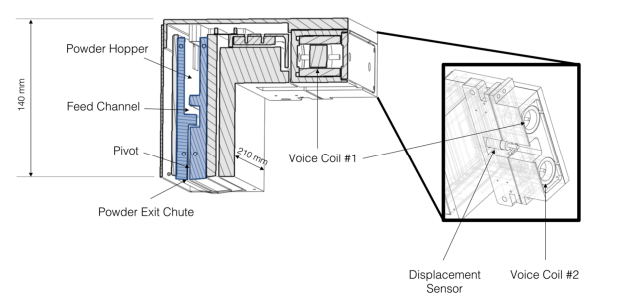
\includegraphics[width=\textwidth]{../report_assets/vibrational_feed.png}
        \caption*{(b) Vibration Fed Design~\cite{Sinclair2021}}
    \end{minipage}
    \hfill
    \begin{minipage}{0.3\textwidth}
        \centering
        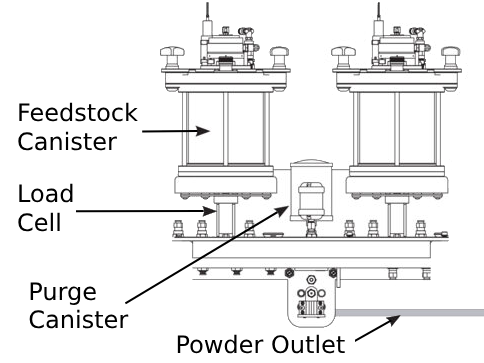
\includegraphics[width=\textwidth]{../report_assets/Liquid_oerlikon.png}
        \caption*{(c) Liquid Suspension Design~\cite{OerlikonMetcoFeeders2023}}
    \end{minipage}

    \vspace{0.5cm} % space between top and bottom rows

    % Second row: 2 images
    \begin{minipage}{0.35\textwidth}
        \centering
        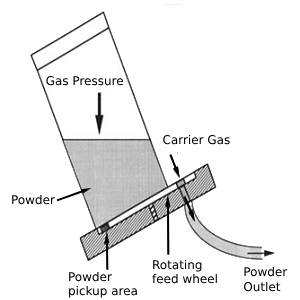
\includegraphics[width=\textwidth]{../report_assets/rotating_disk.png}
        \caption*{(d) Rotating Disk Design~\cite{Crawmer2013}}
    \end{minipage}
    \hspace{0.1\textwidth}
    \begin{minipage}{0.35\textwidth}
        \centering
        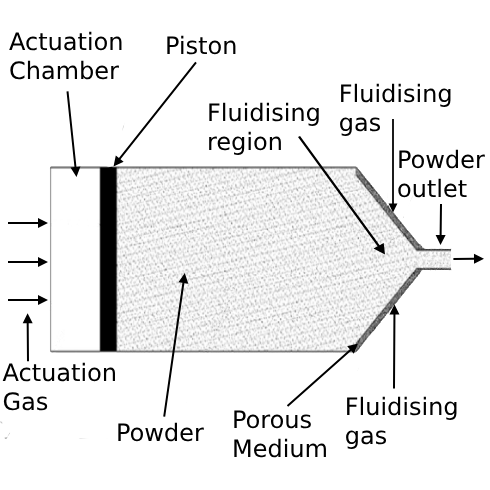
\includegraphics[width=\textwidth]{../report_assets/fluidising_powder_design.png}
        \caption*{(e) Fluidised Powder Bed Design~\cite{Li2016}}
    \end{minipage}

    \caption{5 common powder feed system architectures.}\label{fig:powder-dispensing-methods}
\end{figure}
Given that CSAM already requires an accelerant gas, the fludising powder bed design was deemed the most optimal as this mitigates one of the architectures largest drawbacks. Furthermore, the method is assumed to be inherently gravity-agnostic, requiring no adjustments of the core mechanic of feeding. 

As mentioned in \autoref{sec:fluidised-powder-feed-systems}, the fluidising powder bed architecture has gone through a number of design iterations since it's first implementation. To align the investigation as closely to state-of-the-art, the pneumatically driven, permiable piston architecture was chosen. This also simplifies the systems plumming and reduces the overall mass of the system but comes at the cost of complexity in dynamics.

\section{Hopper Tank Design}
% what it was designed for
The tank was designed to operate at a maximum pressure of 8 bar because of previous experience during the COSMOS project. 8 bar was on the high end of powder hopper inlet pressures during successful tests and was therefore deemed appropriate. A safety factor of 1.5 was chosen but only after manufacturing, it was discovered that the standard for pressure vessels was 3.5-4~\cite{redriver2024asme}. This would be accounted for given another design iteration but was determined a low priority given the time constraints.

% what it was made from and why
The end caps were manufactured from Acetal C POM Delrin as the material is low-cost, easy to machine and chemically inert. The tube was made from clear acrylic to allow the flow behaviour to be observed but upon evaluation, polycarbonate would have been more appropriate as it is less prone to shattering.
% what it looks like
\begin{figure}[htbp]
    \centering

    % First row: 3 images
    \begin{minipage}{0.3\textwidth}
        \centering
        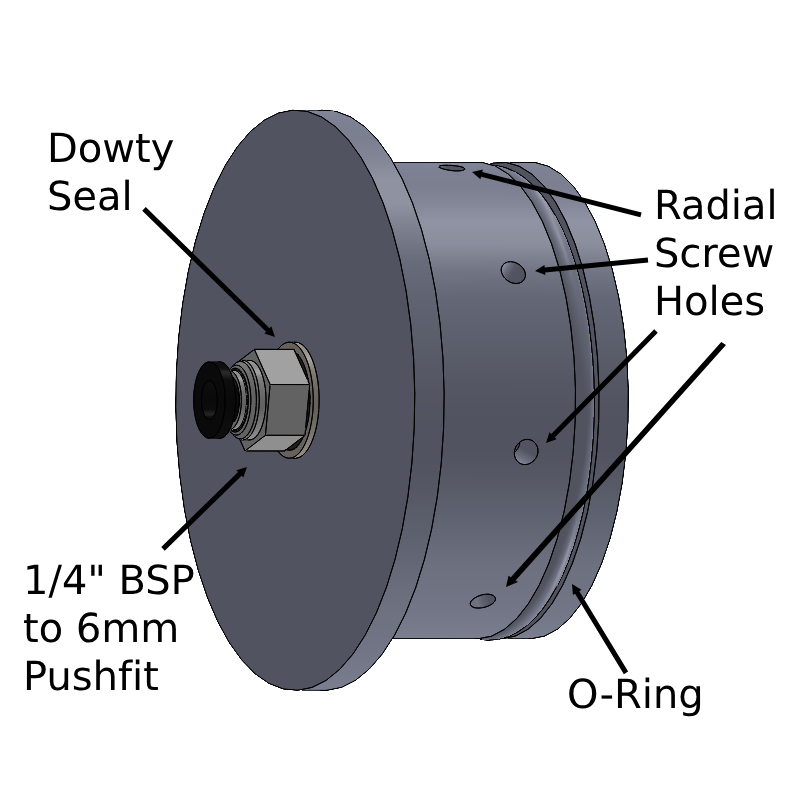
\includegraphics[width=\textwidth]{../report_assets/inlet_end_cap.png}
        \caption*{(a) Inlet End Cap}
    \end{minipage}
    \hfill
    \begin{minipage}{0.3\textwidth}
        \centering
        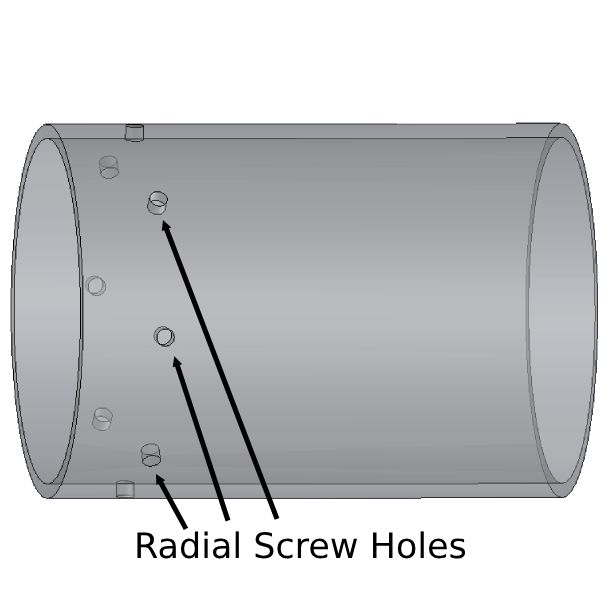
\includegraphics[width=\textwidth]{../report_assets/tube.png}
        \caption*{(b) Acrylic Tube}
    \end{minipage}
    \hfill
    \begin{minipage}{0.3\textwidth}
        \centering
        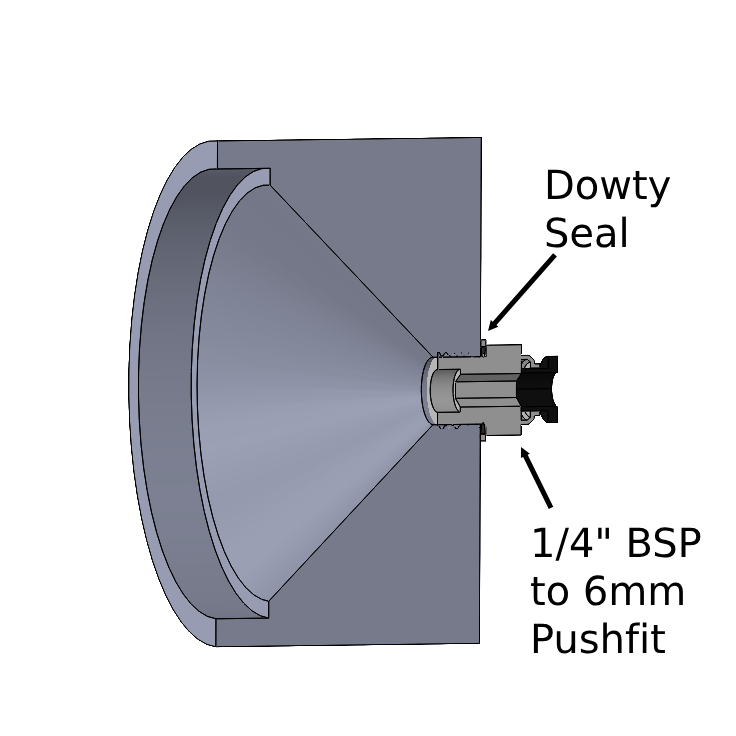
\includegraphics[width=\textwidth]{../report_assets/outlet_end_cap.png}
        \caption*{(c) Outlet End Cap Cross Section}
    \end{minipage}
    \caption{Components of the Hopper Tank}\label{fig:hopper-tank-components}
\end{figure}
As seen in \autoref{fig:hopper-tank-components}, the inlet end cap is radially screwed into the tube. This was done as one of the end caps had to be removable to allow for changing the piston. The outlet end cap was bonded to the tube using plastic-friendly epoxy.

% additional functionality requirements
To validate that the design could operate at a pressure of 8 bar, a combination of hand calculations and finite element analysis (FEA) were conducted. The failure modes analysed were stress concentrations from the bolt holes and hoop stress rupture. Fracturing at the delrin-epoxy interface was a concern but there is no relevant literature on how to model this so it was not investigated. Bolt tearout was not investigated as it was deemed an unlikely mode of failure.

% design evaluation
Upon construction of the tank, it was hydrostatically pressure tested to a pressure of 8 bar. At the time of testing, it was known that the safety factor of the design was lower than standard and therefore was not pressurised above the 8 bar limit for fear of damaging the tank. This was definitely not ideal but given the time and budget constraints, manufacturing a new powder hopper was not an option.

\section{Piston Design}\label{sec:piston}
The piston's main function in this design is to constrain the powder to the outlet of the device. By modelling the sand as a fluid, the force required by the piston to pack the sand against the outlet can be calculated through the hydrostatic pressure equation, seen below. 
\begin{equation}\label{equ:hydrostatic}
P = \rho * h * g
\end{equation}
This pressure has to balance the pressure differential across the piston from the flow and the additional frictional force on the tank walls to ensure the powder is packed at the outlet. Both the modelling of the pressure differential and the friction from the walls was too complex for a first principles driven desing. Therefore the first design, seen in \autoref{fig:piston_geom} (a), was modelled after a previous study which found the gear geometry to have the best performance~\cite{TANG2023118406}. This was 3D printed with PLA and there was a concern that the high pressure within the tank would not equalise with the pressure inside the print causing crumpling. This is why the wall layers were not printed to allow for this equalisation. 
\begin{figure}[htbp]
    \centering

    \begin{minipage}{0.3\textwidth}
        \centering
        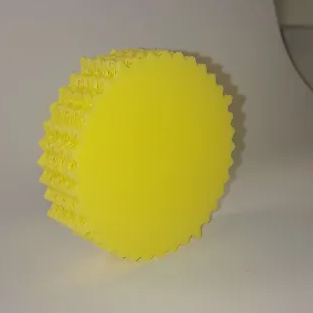
\includegraphics[width=\textwidth]{../report_assets/piston_1.png}
        \caption*{(a) First Design Iteration.}\label{fig:piston_geom_1}
    \end{minipage}
    \hfill
    \begin{minipage}{0.3\textwidth}
        \centering
        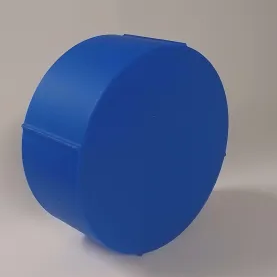
\includegraphics[width=\textwidth]{../report_assets/piston_2.png}
        \caption*{(b) Second Design Iteration.}\label{fig:piston_geom_2}
    \end{minipage}
    \hfill
    \begin{minipage}{0.3\textwidth}
        \centering
        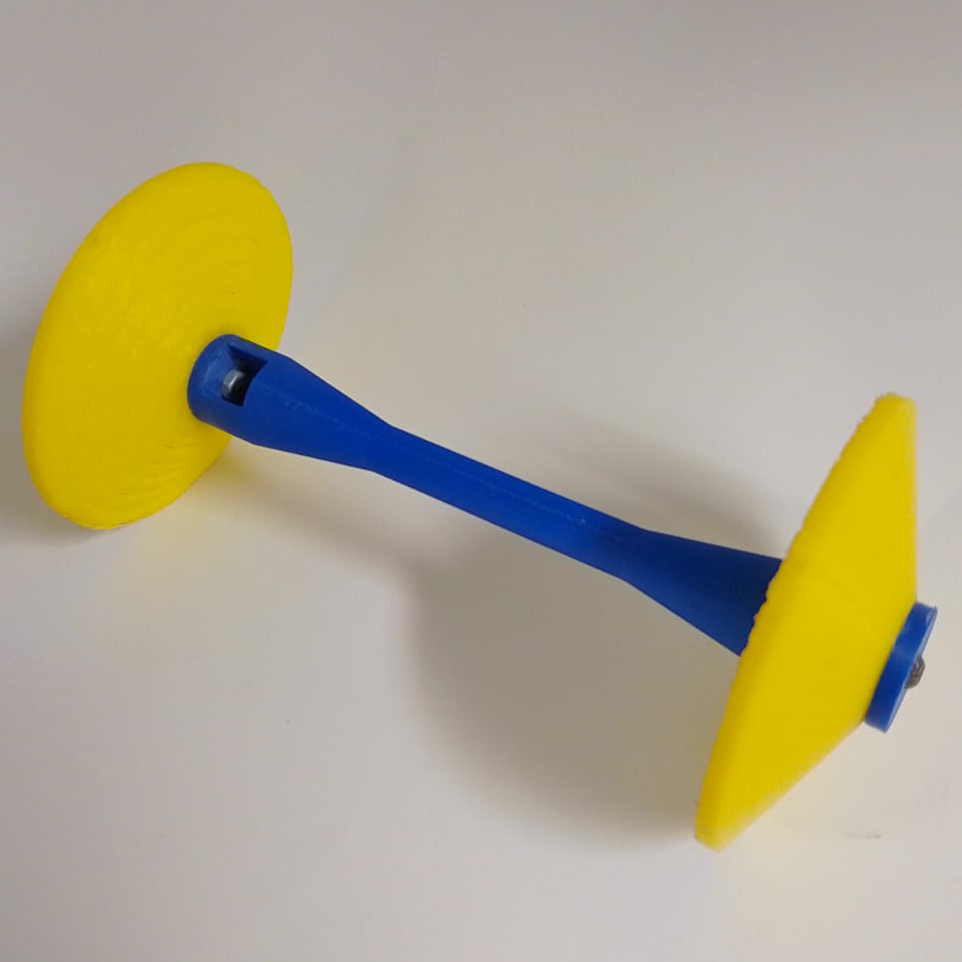
\includegraphics[width=\textwidth]{../report_assets/piston_final.png}
        \caption*{(c) Final Design.}\label{fig:piston_geom_3}
    \end{minipage}
    \caption{Piston Design Iterations}\label{fig:piston_geom}
\end{figure}
The first design did not generate enough pressure force to be moved down the tank, motivating the need for another iteration. Building off this insight, the second piston was designed to try and constrict the flow around the piston as much as possible to generate a higher pressure force. As discussed in \autoref{sec:first-test}, this piston did move from the pressure but immediately became jammed by the sand. This motivated the next redesign, using a new paradigm to prevent the piston from jamming. The final piston consists of 2 3D printed TPU cones and a connecting rod. The flexibility of the TPU provided much needed resiliance against jamming as individual grains could be flexed around or over to continue compacting the rest. Another common solution to prevent piston cocking is to make it longer and this was achieved through the blue rod. Not only did this allow for the piston to be lighter weight than a fully TPU piston, it also allowed each face to be thinner and therefore give less contact area for friction or powder jamming. Furthermore, the piston face could fully cover the cross section of the tank due to the resistance to sticking and permiability of the print, allowing for a higher pressure differential and, in turn, more consistent compaction of the sand against the outlet.

% In the permiable piston architecture, this is achieved through a constricting the flow to create a pressure differential across the two faces and therefore a resultant force pushing on the piston which is pushing on the powder. One way to do this is through reducing the gap between the tank wall and sides of the piston as it decreases the flowrate passed the piston, allowing the static pressure to build. However, the smaller the gap between the two surfaces, the higher the frictional forces and the increased likelyhood that sand grains get between the two surfaces and further increase friction. This resulted in 3 different geometries being tried.
% The first was blah blah blah and was used in testing the system for the first time.
% Upon identifying that this was not pushing the piston far enough, the piston was redesigned taking inspiration from cite the gear paper.
% This then ran into the issue of cocking, a problem where the piston becomes misaligned due to pressure differences.
% The final design was then proposed to solve both the issue of higher dp requirement and cocking/powder sticking resistance. This was made using TPU as it is flexible enough to warp around particles that would otherwise dig into the PLA pistons, and strong enough to hold back most of the air. Due to manufacturing imperfections, the prints had a high surface roughness and measuring permiability of the piston would be done given more time.
\newpage

\section{Expected Behaviour}
While there are few investigations into the specific implementation of the fluidising bed, parallels can be drawn from similar systems. It has been proposed that you can split the analysis of the flow behavior within the tank into two regions: a dense phase moving area before the cone and a fluidising region afterwards~\cite{Tang22}. This analysis assumes arching occurs, seen in \autoref{fig:bulk_powder_structures}, due to the presence of the tube cone interface and pressure from the piston restricting powder movement. This constrains the flows movement above the interface and [maybe means there is no correlation between force on powder and flow rate]

lower pressure due to not needing to go into combustion chamber
% \begin{figure}[htbp]
%     \centering

%     \begin{minipage}{0.3\textwidth}
%         \centering
%         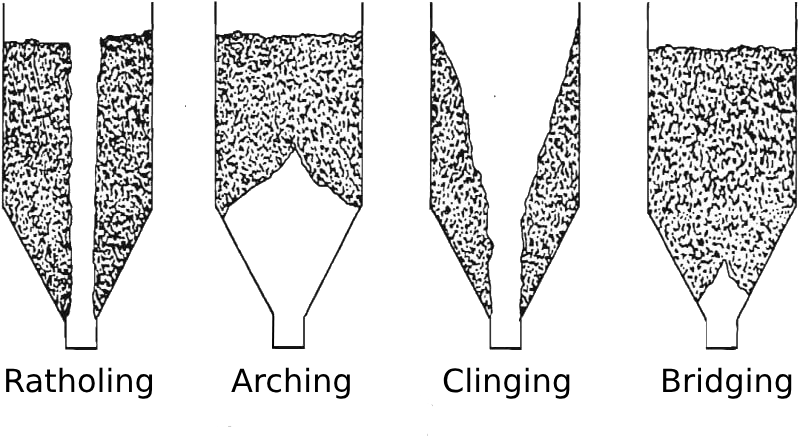
\includegraphics[width=\textwidth]{../report_assets/bridging.png}
%         \caption{Bridging ig\cite{911Metallurgist_binsflow}.}
%     \end{minipage}
%     \hfill
%     \begin{minipage}{0.3\textwidth}
%         \centering
%         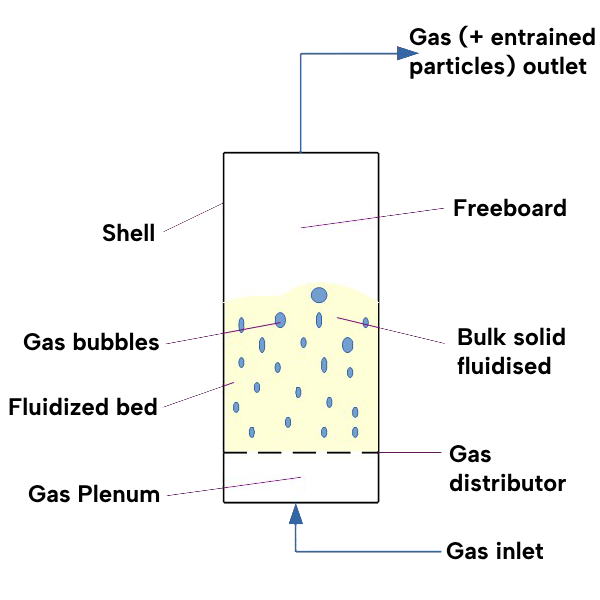
\includegraphics[width=\textwidth]{../report_assets/Fluidised_Bed_polished.png}
%         \caption{Simplified fluidised powder bed diagram.}
%     \end{minipage}
%     \hfill
%     \begin{minipage}{0.3\textwidth}
%         \centering
%         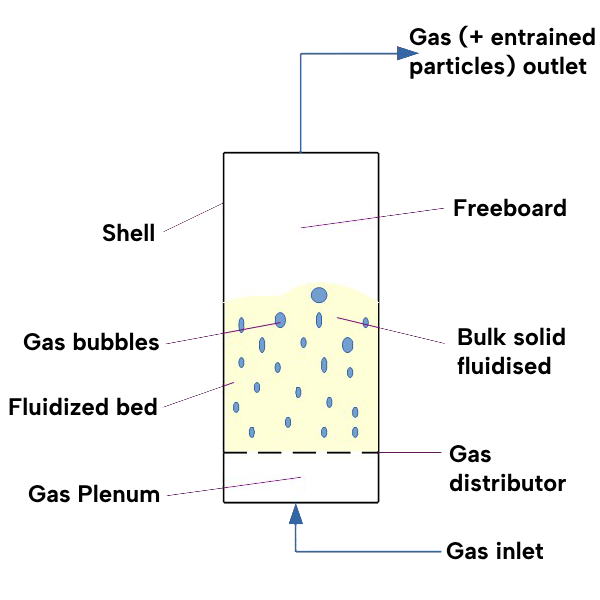
\includegraphics[width=\textwidth]{../report_assets/Fluidised_Bed_polished.png}
%         \caption{Current design with turbulent inlet.}
%     \end{minipage}
%     \caption{i dont know yet}\label{fig:idknowyet}
% \end{figure}
% Given that the architecture is a revision of older systems, it is analysed in two stages. Like the motor-actuated 
% One could expect to model a system like this by combining previous data and insight of how the motor actuated fluidised system works and then augmenting this due to the pneumatic actuation of the piston. However, previous investigations into this [cite] seem to suggest that there is no such correlation between force applied to the piston and mass flow rate of the powder. 

% \begin{figure}[htbp]
%     \centering

%     \begin{minipage}{0.3\textwidth}
%         \centering
%         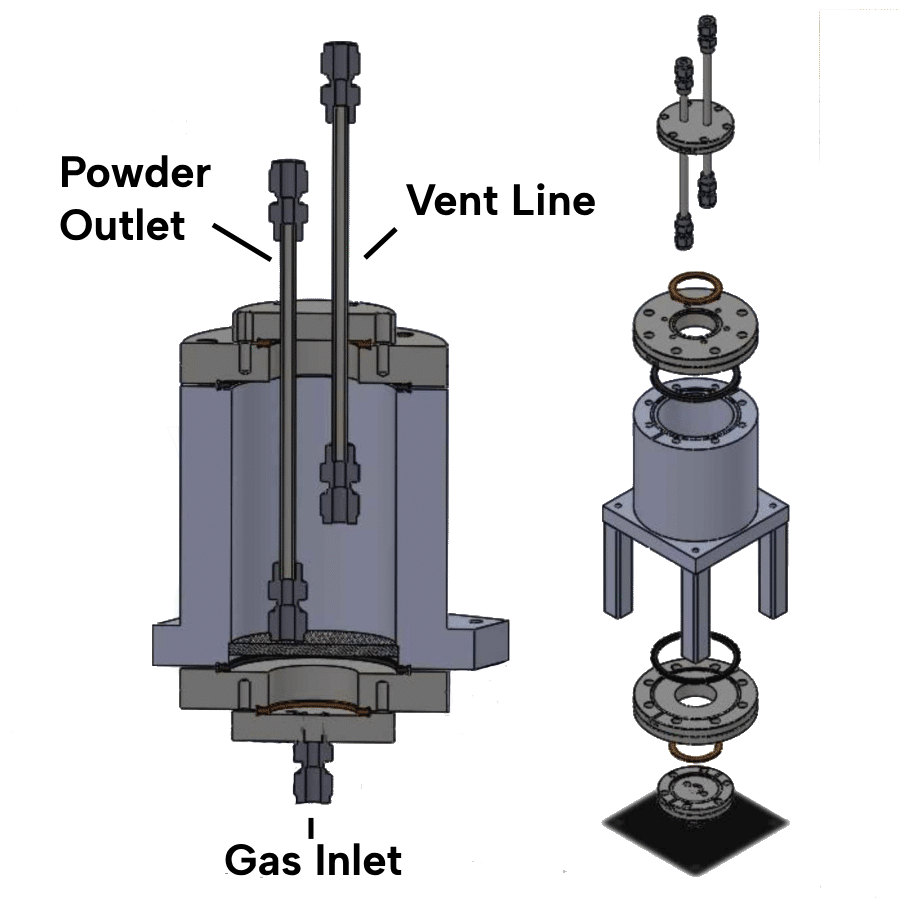
\includegraphics[width=\textwidth]{../report_assets/COSMOS_DIAGRAM.png}
%         \caption{Current feed system diagram.}\label{fig:idkyet1}
%     \end{minipage}
%     \hfill
%     \begin{minipage}{0.3\textwidth}
%         \centering
%         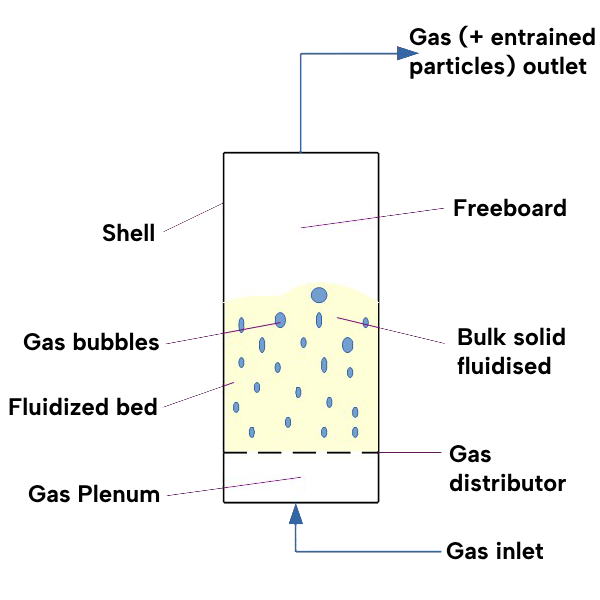
\includegraphics[width=\textwidth]{../report_assets/Fluidised_Bed_polished.png}
%         \caption{Simplified fluidised powder bed diagram.}\label{fig:idkyet2}
%     \end{minipage}
%     \hfill
%     \begin{minipage}{0.3\textwidth}
%         \centering
%         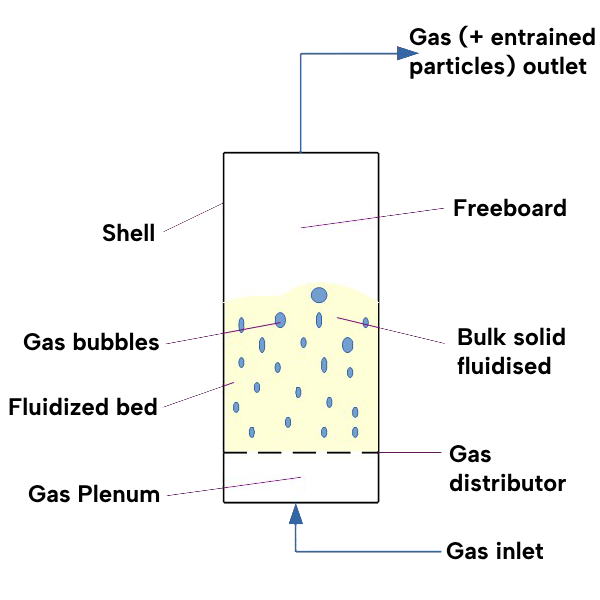
\includegraphics[width=\textwidth]{../report_assets/Fluidised_Bed_polished.png}
%         \caption{Current design with turbulent inlet.}\label{fig:idkyet3}
%     \end{minipage}

% \end{figure}
% It is expected that this is because the PT is too far downstream and the powder inbetween is lowering the pressure. Using data given for the experimentation and the pressure drop expected from the cylindrical powder section alone
% it has previously been reported that there is not a simple linear relationship between the force of the piston on the powder and the 

% % lowkey weak argument look for better

% Another argument about piston force VS mass flow rate

% alternatively there is a strong linear correlation between velocity of piston head and mass flow rate of powder. This is well defined and could be used instead of the force


% The physics is hopefully understood as a non-linear combination of the two effects. Gas applying a force to the piston and the fluidisation of the powder. If we look at the system as though it is not gas permiable then we would expect it to look like this. Given the piston head is though, we expect it to change in this way.

% At the end of the day, this system is similar to other systems investiaged. It varies in 1 key way, the fact that since it is going into a nozzle then a vacuum in the LPCS process there is no combustion chamber to provide backpressure.
% \newpage

\section{Experimental Setup}
The experimental set up was designed to verify the expected behaviour of the fluidising powder feed system under terrestrial conditions to better estimate it's behaviour under microgravity. The core aims were to record the consistency of the powder mass flow rate, verify that changing the pressure upstream of the tank leads to a change in mass flow rate and document any behaviours the system may exhibit that would impact it's suitability for space applications.

\subsection{Layout}
The default layout, seen in \autoref{fig:experimental-setup}, was used to perform most of the testing, with modifications outlined in the sections where they occur. 
\begin{figure}[htbp]
    \centering

    \begin{minipage}{0.6\textwidth}
        \centering
        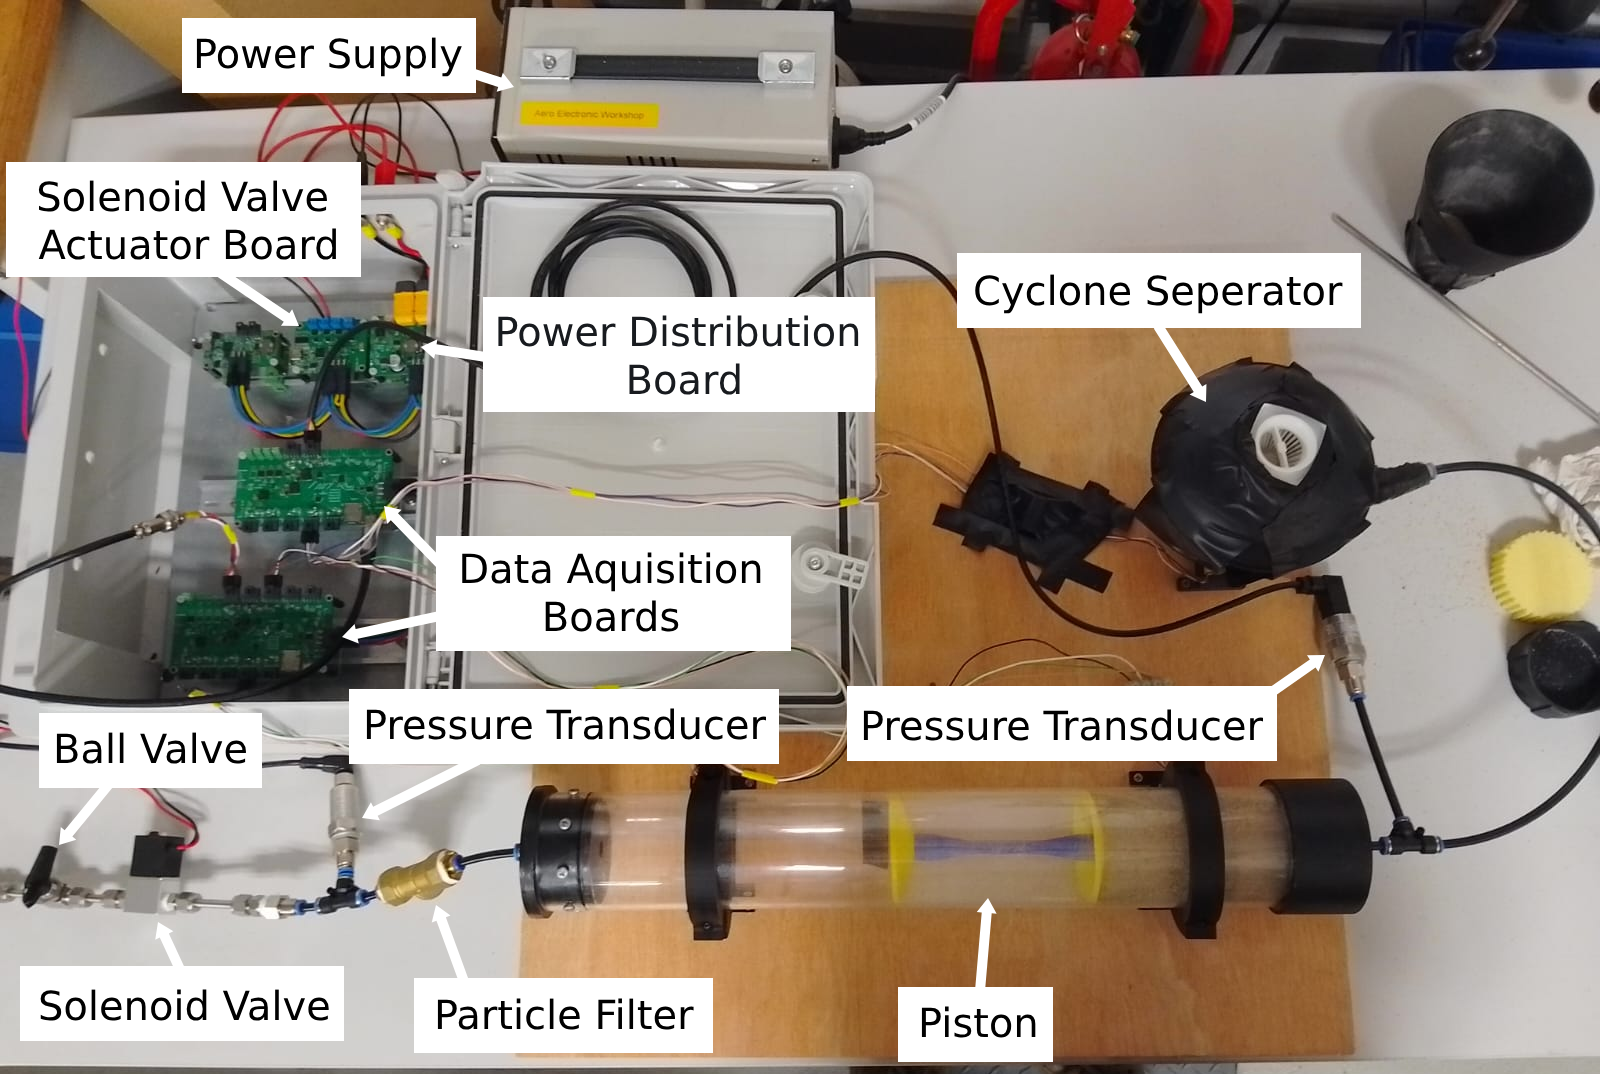
\includegraphics[width=\textwidth]{../report_assets/setup_annotated.png}
        \caption*{Annotated Image of Setup}
    \end{minipage}
    \hfill
    \begin{minipage}{0.3\textwidth}
        \centering
        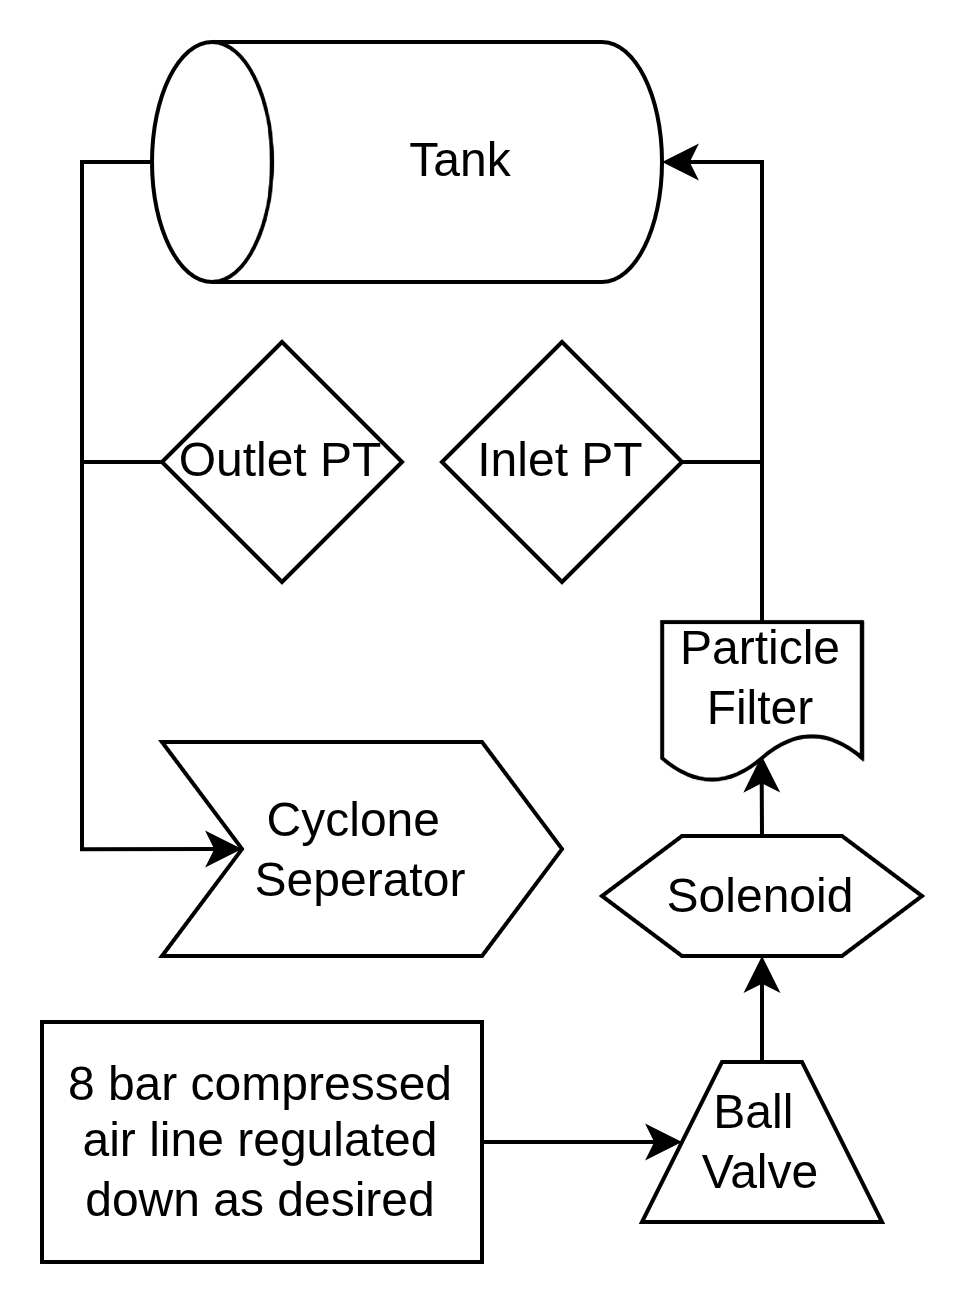
\includegraphics[width=\textwidth]{../report_assets/drawio_setup_vertical.png}
        \caption*{Systems Diagram of Setup}
    \end{minipage}
    \caption{Experimental Setup}\label{fig:experimental-setup}
\end{figure}
The testing was undertaken inside Imperial College's Hypersonic Lab which maintains no climate control. It was assumed that the system would not behave noticeably differently under the slightly varying teperatures and pressures that occured over the testing.

\subsection{Data Acquisition and System Actuation}
To capture the system's behaviour, a combination of video recordings, load cell readings and pressure transducer readings were taken during each test. The placement of the sensors is shown in \autoref{fig:sensors} and their values were read with the use of custom electronics designed by the Imperial College London Rocketry team.
\begin{figure}[htbp]
    \centering

    \begin{minipage}{0.45\textwidth}
        \centering
        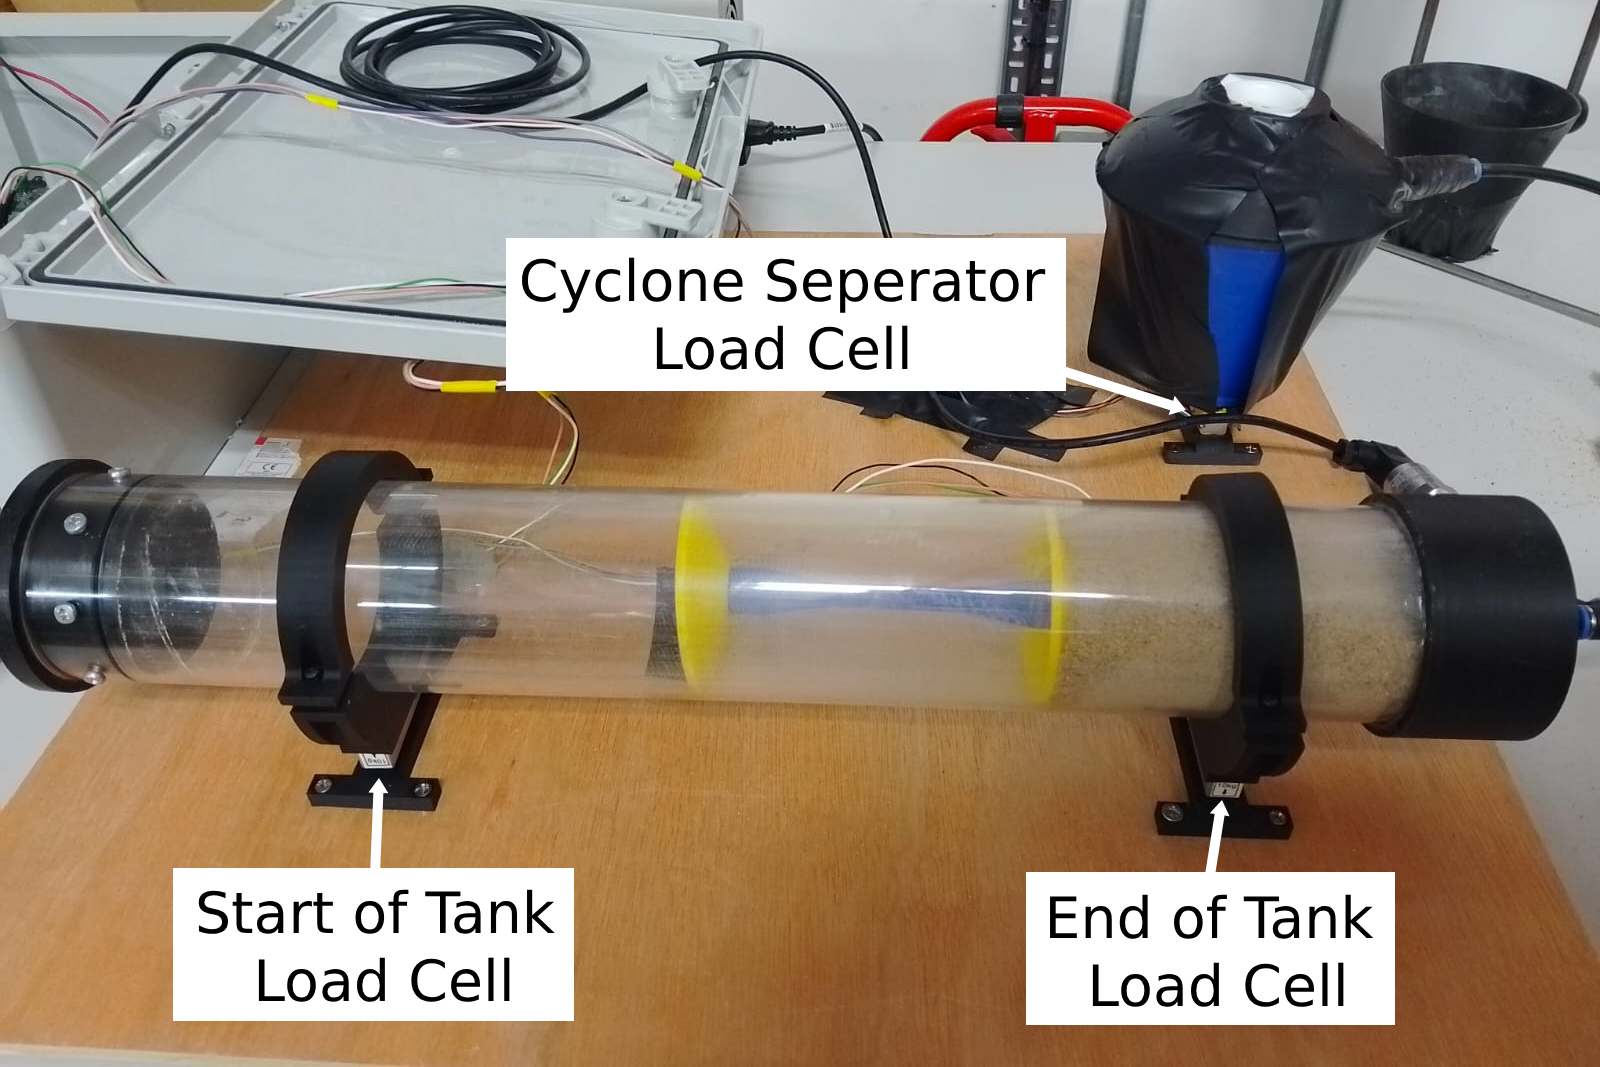
\includegraphics[width=\textwidth]{../report_assets/load_cell_configuration.png}
        \caption*{Load Cell Placement}
    \end{minipage}
    \hfill
    \begin{minipage}{0.45\textwidth}
        \centering
        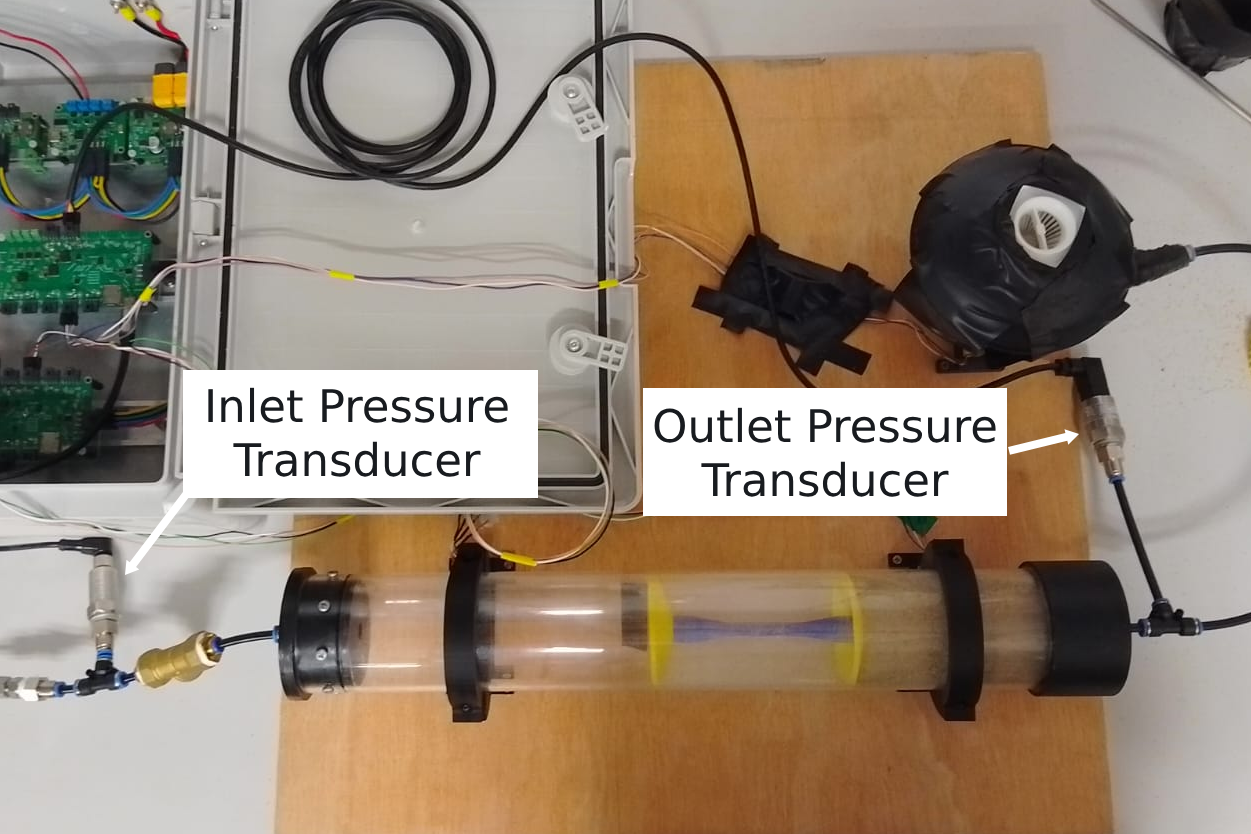
\includegraphics[width=\textwidth]{../report_assets/pressure_transducer_configuration.png}
        \caption*{Pressure Transducer Placement}
    \end{minipage}
    \caption{Sensor Placement in Experimental Setup}\label{fig:sensors}
\end{figure}

A computer was connected to the boards and data was logged to it as well as being presented on a bespoke user interface, shown in \autoref{fig:grafana}. The solenoid could also be opened and closed through the dashbaord, allowing for safe operations as all the information and control was in one place.
\begin{figure}[htbp]
    \centering

    \begin{minipage}{0.95\textwidth}
        \centering
        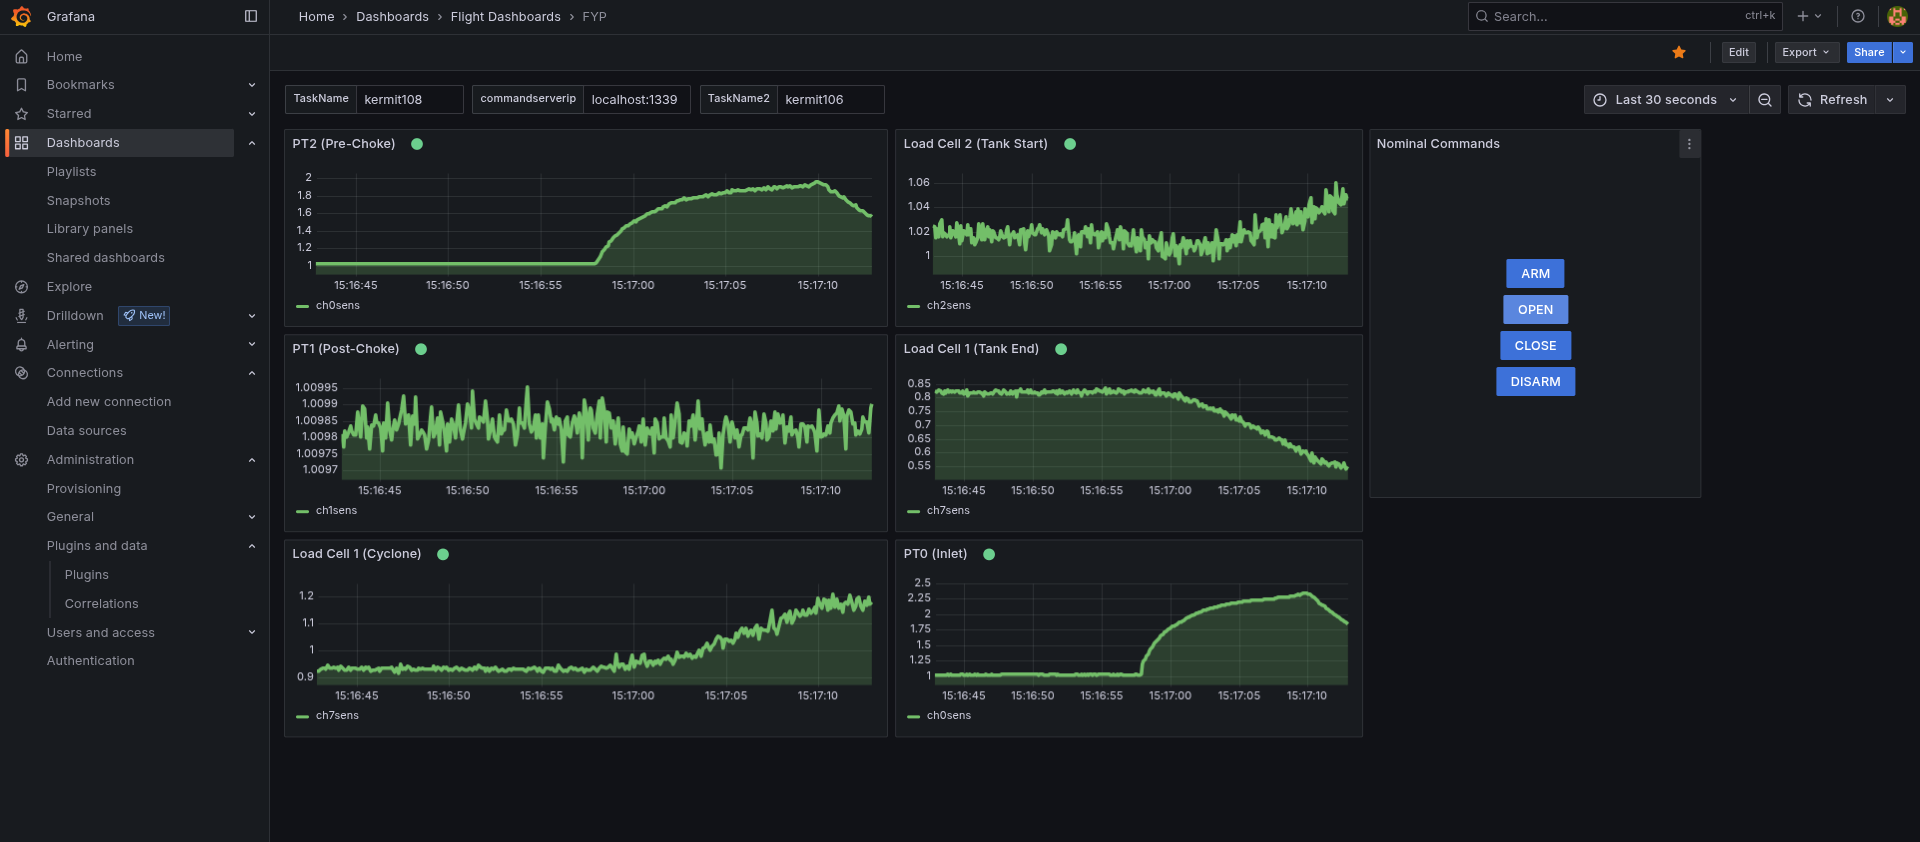
\includegraphics[width=\textwidth]{../report_assets/grafana.png}
        \caption{Testing Dashbaord}\label{fig:grafana}
    \end{minipage}

\end{figure}
Due to budget constraints only cheap pressure transducers and load cells were used. Given this, perfect calibration of the sensors was not as much of a priority. To calibrate the load cells, the data aquisition baord was configured to record the raw values out put by the analog to digital converter (ADC) at both the unloaded, 0kg, state and then with a mass, measured at 0.746kg, placed on it. Since the load cells are a linear sensor, these two points give a gradient and y-intercept to map the ADC counts to. The same procedure was done to calibrate the pressure transducers except using a mechanical pressure gauge and the compressed air line to record 1bar and 4bar ADC outputs.

An older setup of the experiment included a choke point just after the outlet of the tank. This was because previous literature proposed that fluidising systems where one part of the gas-solid flow is in choking conditions had been found to be simpler to control~\cite{SUN201630}. Due to the grain size of the sand, this chokepoint got clogged in testing so was removed. As there was a pressure transducer before and after the chokepoint, this explains the naming scheme in \autoref{fig:grafana} and why the pre-choke pressure data is just noise as it was no longer connected.

\subsection{Cyclone Seperator and Measurement Method}
The two most common methods of measuring mass flow rate for this kind of system are using a displacement transducer to measure how far down the tank the piston is or measuring the mass of the powder after it has been fed out of the tank~\cite{SUN201630}\cite{LI2021712}\cite{Tang22}.
 The displacement transducer method indirectly measures the mass flow by using the near incompressibility of the powder and the assumption of a constant packing density to form a linear relationship between the movement of the piston and the volume of powder dispensed~\cite{SUN201630}. The direct method requires some method of seperating the gas and powder and then measures the powder. 

WHY dID I CHOSE THE SEPERATOR INSTEAD OF THE Displacement
EDITS TO TANK UNIDEAL GIVEN PRESSURE RATING things
NEED TO CAPUTRE AIR ANYWAY FOR HEALTH AND SAFETY SO EASIER TO implement
MAYBE CITE COMPARISON PAPER

To seperate the gas and powder, a cyclone seperator was used, seen in \autoref{fig:cyclone}.
\begin{figure}[htbp]
    \centering

    \begin{minipage}{0.3\textwidth}
        \centering
        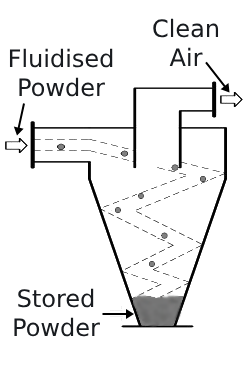
\includegraphics[width=\textwidth]{../report_assets/cyclone_diagram.png}
        \caption*{(a) Cyclone Seperator Diagram}
    \end{minipage}
    \hfill
    \begin{minipage}{0.3\textwidth}
        \centering
        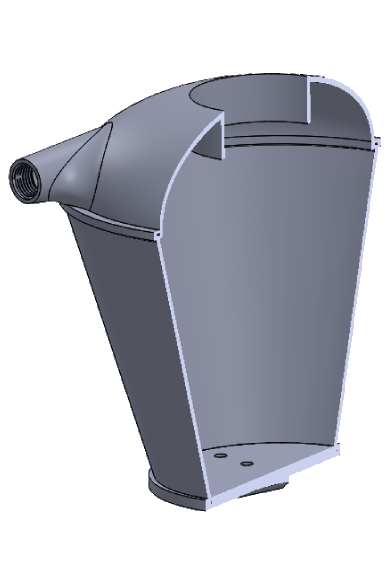
\includegraphics[width=\textwidth]{../report_assets/cyclone_cad.png}
        \caption*{(b) CAD Model of Seperator}
    \end{minipage}
    \hfill
    \begin{minipage}{0.3\textwidth}
        \centering
        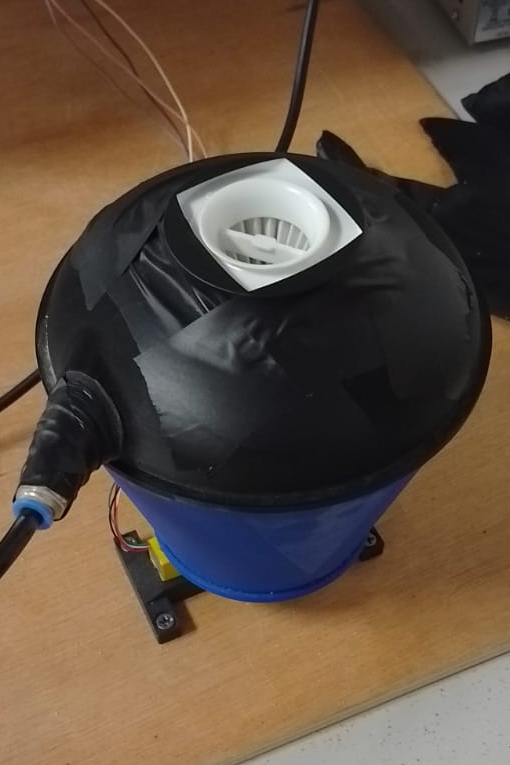
\includegraphics[width=\textwidth]{../report_assets/cyclone_done.png}
        \caption*{(c) Cyclone Seperator}
    \end{minipage}
    \caption{Sensor Placement in Experimental Setup}\label{fig:cyclone}
\end{figure}
A cyclone separator works by using centrifugal force to separate the sand from the air. As the mixture enters the cyclone chamber tangentially at high speed, it spins rapidly, causing the denser particles to move outward and fall to the bottom, while the cleaner air exits through the top center. As shown in \autoref{fig:cyclone} (c), a dust filter used in vacuum cleaners was used to ensure any fine grains, not captured by the seperator, do not make it out into the air. This was attached to the 3D printed model using PTFE tape and a friction fit, then taped down for added support. The seperator was printed in 3 parts, the top that can be removed to empty out the sand, the walls and the base with screw holes to mount to the load cell.
% The direct cyclone seperator method was chosen to record mass flow, with a back up recording of the mass of the tank during operations. This is because the sand needs to be contained after exiting the tank as inhalation of silica particles can lead to long term health conditions. Therefore, the direct method was chosen as

\subsection{Powder}
While typical powders used in CSAM are $5\,\mu\mathrm{m}$ to $100\,\mu\mathrm{m}$~\cite{Vaz2023}, budget constraints resulted in sand being the optimal granular material safe enough to work with. This will definitely affect the behaviour of the system but to what extent is unknown. A rudimentary attempt was made to measure the particle diameter using a micrometer but given the time limitations, no formal attempt was made to characterise the diameter distributions or average diameter. As mentioned in \autoref{sec:numerical-setup}, the bulk density, that being the density of the sand including the volume occupied by air, was measured by recording the mass of the sand in a bowl and then filling the same bowl with water.

% For safety and due to the limited budget, sand was used as the powder. This is one of the greatest areas for improvement, i dont actually know what size the powder is or the distribution of those sizes. This powder has been measured to have [density = 1.4g/cm3]

% \newpage

\subsection{Procedure to Characterise Pressure Source}
Due to safety and ease of handling, the desired stagnation pressure supplied into the system came from a compressed air line. As discussed in \autoref{sec:static_test}, characterising the air supply was not trivial and required multiple experiments. 

The first of these involved a flow through the system without any sand or piston. To tune the regulator for these tests, the system was closed by removing inlet tube connecting the tank to the compressed air line and replacing it with a pushfit end cap, as seen in figure \autoref{fig:systems-diagram-end-cap}. The regulator attached to the compressed air line was then adjusted using the inlet PT as a reference. While there was a gauge on the regulator, it was consistently reading 0.2 to 0.3 bar higher than the PTs or manual pressure gauges so was deemed unreliable. 
\begin{figure}[htbp]
    \centering
    \begin{minipage}{0.45\textwidth}
        \centering
        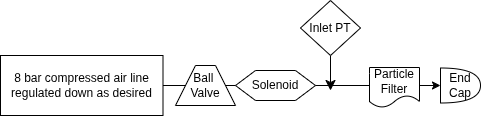
\includegraphics[width=\textwidth]{../report_assets/end_cap.drawio.png}
        \caption{Diagram of closed system.}\label{fig:systems-diagram-end-cap}
    \end{minipage}
\end{figure}

Once the pressure was tuned on the regulator, the ball valve was closed, the end cap was removed and the tube was reattached to the tank. The system was now back to it's open configuration and the static pressures were read by opening the solenoid valve allowing the air to flow.

Follow up tests were conducted to validate that the test set up was not configured incorrectly. The static pressure readings were abnormally low and this could have been attributed to many things. The most likely and therefore first investigated was the pressure regulator. If the regulator was faulty or there was somehow dramatic static pressure losses from the outlet of the compressed air line to the inlet of the ball valve this could be remedied by adding an additional regulator after the ball valve and fully opening the one connected to the wall.
The same tests as before were conducted to investigate this but the static pressures read were even lower suggesting this wasnt the issue.
A final attempt to solve the problem was verifying that the solenoid valve wasn't causing the problem. If the cross-sectional area of the open solenoid valve was very small, this could have choked the flow and lead to the lower stagnation pressure observed. Even after running the same test again without the solenoid valve, the results were equal to that of the system with the regulator and solenoid valve.

% To further investigate this behaviour, the pressure regulator connected to the compressed air line was set to max (roughly 7bar) and a second regulator was introduced closer to the system. If the problem was large static pressure losses from the long nylon tube connecting the inlet of the experiment to the pressure source, a larger pressure during operation would have been observed. Additionally, if the pressure regulator was faulty or some other weird behaviour was occuring upstream of the setup, this could have indicated that.
\subsection{Procedure to Characterise Full System}

\newpage
\section{Numerical Setup}\label{sec:numerical-setup}
\subsection{Numerical Setup to Characterise Pressure Source}
To verify the source pressure behaviour seen in \autoref{sec:static_test} a 2D, axisymmetric simulation of the simplified system was ran. The geometry used and something can be seen In
\begin{figure}[htbp]
    \centering

    \begin{minipage}{0.45\textwidth}
        \centering
        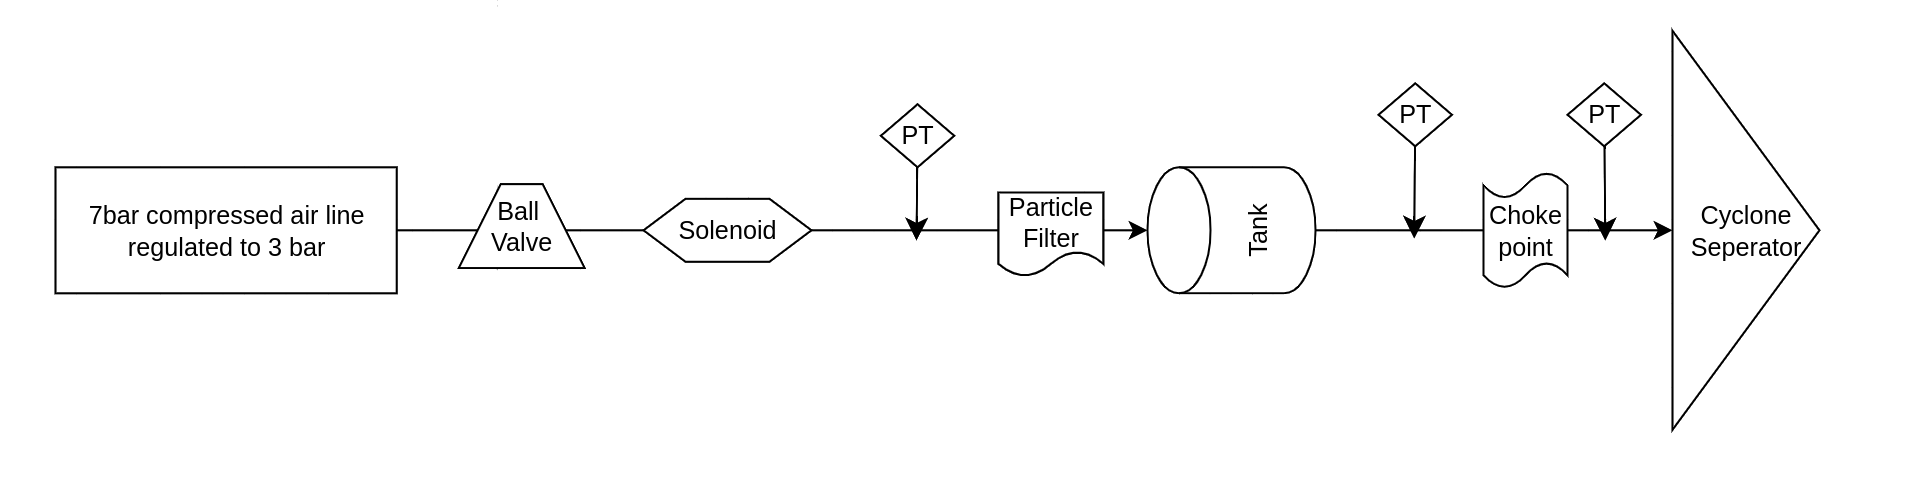
\includegraphics[width=\textwidth]{../report_assets/systems_diagram.png}
        \caption{Systems diagram.}\label{fig:geometry_static_sim}
    \end{minipage}
    \hfill
    \begin{minipage}{0.45\textwidth}
        \centering
        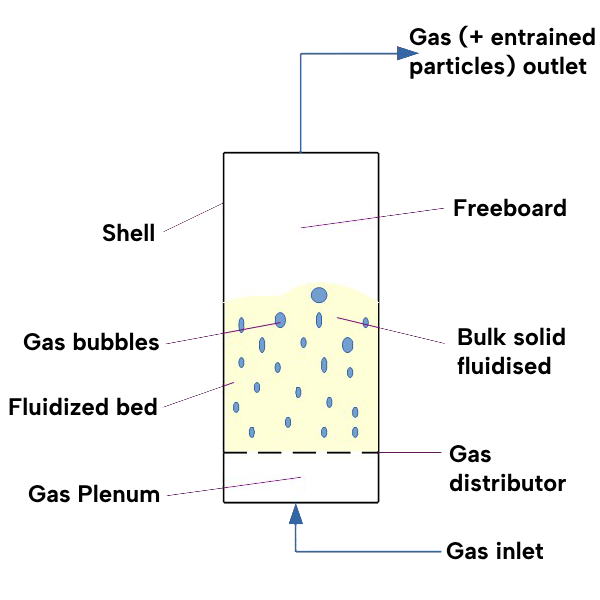
\includegraphics[width=\textwidth]{../report_assets/Fluidised_Bed_polished.png}
        \caption{Pic of experiment.}\label{fig:something_else}
    \end{minipage}

\end{figure}
and was done as a 2D, axisymmetric sim as it was faster and allowed for more detail while still preserving quantities of 3D behaviour as no theta dependence or swirling is expected to occur. Size constraints on the number of cells meant that all attempts to invesitage a 3d sim of the physics were numerically unstable and therefore werent useful.

Mesh convergence was done maybe if i got time?
\subsection{Numerical Setup to Characterise Full System}

% \subsection{Moving piston simulation}
% governing equations eularian-eularian
% 2d is valid because:
% 2D vs 3D Eulerian Multiphase Simulations of a Piston-Driven Fluidised Bed
% Flow Features in 2D vs 3D Multiphase Models
% Hydrodynamics and Void Distribution: Two-dimensional Eulerian-Eulerian simulations can reproduce many qualitative behaviors of fluidised beds, but they often differ quantitatively from three-dimensional models. A key issue is that 2D models tend to over-predict void fractions and bed expansion, especially at higher flow velocities
% link.springer.com
% . This occurs because neglecting the third dimension forces the gas-solid flow into a constrained plane, which exaggerates hydrodynamic structures and fluctuations
% link.springer.com
% . In practical terms, a 2D simulation may show larger void regions (bubbles) and more vigorous oscillations in solid concentration than a real 3D system would. These differences mean that certain flow features are not identical between 2D and 3D:Bubble Dynamics: Gas bubbles in a fluidised bed behave differently in a 2D domain. Studies have found that bubbles remain smaller and rise more slowly in a 2D (pseudo-2D) bed than in a full 3D bed
% witpress.com
% . In a 3D simulation or experiment, bubbles can expand and coalesce in three directions, forming larger voids that accelerate upward. The 2D constraint suppresses some coalescence, so the bed may appear “bubblier” (many small bubbles) or even form slugging bubbles that span the width. This impacts particle motion and could alter the paths through which solids circulate and exit the bed.
% Circulation and Wall Effects: Three-dimensional beds allow complex circulation patterns — particles can move around bubbles and across the entire cross-section. In a 2D model, by contrast, flow is essentially confined between two parallel walls (the front and back of the 2D slice). This artificial confinement increases wall friction effects and creates a large circulating cell in the 2D plane that has no out-of-plane escape. As a result, 2D simulations may produce stronger single circulation loops or jetting along the centerline, whereas a 3D bed would have more distributed flow paths (including around the perimeter of bubbles or toward the center of a cylinder). Such differences could influence how continuously and evenly the powder flows out — 3D systems tend to have more uniform, axisymmetric flow, while 2D systems might exhibit more pronounced channeling or periodic “puffing.”
% Turbulence and Mixing: The restriction to two dimensions also affects turbulence and mixing of the phases. Fully 3D turbulent eddies and clusters cannot form in a 2D plane, so 2D simulations often show greater oscillatory behavior (numerical instability or large-scale swings) but less of the small-scale chaotic mixing present in 3D
% link.springer.com
% . For example, pressure fluctuation spectra differ: only a 3D simulation can capture realistic pressure dynamics, whereas a 2D model gives a distorted spectrum
% witpress.com
% . This means the distribution of particles and the stability of the fluidization can differ — a 3D bed might self-buffer some fluctuations by distributing them in all directions, while a 2D bed tends to amplify fluctuations within its constrained geometry.
% Implications for Mass Flow Features: These flow-feature disparities imply that certain phenomena affecting mass outflow could differ between 2D and 3D. For instance, jetting and channeling of powder-gas mixture might be more pronounced in one case versus the other. A 3D piston-driven bed could develop a roughly axisymmetric flow of powder out of the piston region, whereas a 2D model might produce a sheet-like ejection that interacts differently with the walls. Likewise, particle distribution in 3D may be more uniform across the cross-section of an outlet, while in 2D it might be clumped or stratified, potentially affecting instantaneous mass flow rates. Overall, 2D models capture the qualitative flow patterns (e.g.fluidization regimes, general trends in circulation), but certain 3D-specific effects (like true spatial distribution of particles, or the full spectrum of bubble sizes) are lost, which can influence the accuracy of mass flow predictions
% witpress.com
% witpress.com
% . Researchers therefore caution that 2D CFD results should be used primarily for sensitivity studies or trend analysis, whereas 3D simulations are needed to accurately reproduce absolute measures like bed expansion, bubble size distributions, and pressure oscillation characteristics
% witpress.com
% witpress.com
% . In short, 2D and 3D models can differ in circulation patterns, particle clustering, wall friction effects and turbulence - all of which may affect the steady powder outflow rate.
% Linearity of Piston Velocity vs. Powder Mass Flow Rate
% Experimental Observation: In piston-driven fluidised beds (such as pneumatic powder feeders or powder-fueled engines), experiments consistently show that the powder mass flow rate increases approximately linearly with piston velocity (or with related parameters like the throttle/orifice opening)
% researchgate.net
% . Essentially, driving the piston faster injects a larger volume of gas-solids mixture per unit time, yielding a higher mass flow. This linear relationship holds as long as the system is operating below any choking or saturation limits. For example, one study of a powder fuel feeding system found a “high linear tendency” between the mass flow rate and the minimum throttle area (which correlates with piston drive conditions), within the tested range
% researchgate.net
% . Such linear scaling is a fundamental expectation for a displacement-driven flow. 2D Simulation vs 3D Reality: A well-configured 2D Eulerian-Eulerian simulation should qualitatively preserve this linear trend. If the piston (modeled perhaps as a moving wall or boundary in Fluent) is run at different velocities in a 2D model, one would observe that the outflow of powder increases proportionally. In fact, simplified models often treat the piston-induced flow like a controlled volumetric flow rate, which inherently is linear with piston speed in the absence of complex losses. The key question is accuracy: whether the 2D model’s slope of the mass flow vs. velocity curve matches that of a real 3D system. Geometric constraints can introduce some error here. For instance, 2D simulations, by overestimating void fraction and ease of fluidization, might predict slightly higher mass flow for a given piston speed than a 3D simulation or experiment would
% link.springer.com
% . This is because the 2D model may fluidize the powder bed more readily (bubbles percolating easily in the planar slice), offering less resistance to the piston. On the other hand, certain flow resistances (like friction along side walls or limitations in cross-sectional expansion) in 2D could also cause underestimation in some regimes. Notably, discrepancies are expected to grow at more extreme velocities or flow rates. Xie et al. found that when gas velocities are high, the divergence between 2D and 3D models becomes significant - 2D could not satisfactorily predict the hydrodynamics observed in a 3D cylindrical bed
% link.springer.com
% . By contrast, at lower velocities (milder fluidization), 2D and 3D results were more similar
% link.springer.com
% . Translating this to a piston-driven scenario: at modest piston speeds (near the linear operating regime), a 2D simulation will likely yield a linear mass flow response very close to reality. However, as piston velocity increases (approaching choking flow or very aggressive fluidization), the 2D model might deviate - for example, it might fail to capture the onset of non-linearity or throughput limitations that a 3D system would experience. Real 3D systems can develop complex flow distribution (e.g. some regions flowing while others channel or form stagnant zones) at high rates, whereas a 2D model may either over-homogenize this or exhibit unphysical oscillations. Thus, while the linear relationship itself is likely to appear in 2D simulations, the fidelity of its slope and any departure at extremes must be treated with caution. Validation against 3D data or correlations is advised if one plans to use 2D results for quantitative predictions of mass flow.
% Reliability of 2D Predictions and Use in Design
% Early-Stage Design Use: Despite their limitations, 2D multiphase simulations are widely used in early design and feasibility studies because they are much less computationally intensive than 3D models. Importantly, they capture the basic trends and physics of the system, which is often sufficient for preliminary performance estimates. As noted in a recent review, for certain applications like preliminary thermodynamic design or scouting different operating conditions, the more complex 3D approach “does not offer significant benefits” over 2D in terms of high-level outcomes
% link.springer.com
% . The core behaviors - e.g. how increased piston speed affects flow, or how changes in gas feed influence fluidization - are reflected reasonably well in 2D. In fact, 2D simulations can be effectively utilized to illustrate behavioral trends, albeit with some “acceptable disadvantages” such as misrepresentation of exact bed expansion
% link.springer.com
% . In the context of a piston-driven powder bed, a 2D Fluent model would be a theoretically sound and practically convenient tool to predict whether, say, doubling the piston velocity doubles the powder delivery rate (and it likely will show that linear doubling trend). This helps an engineer get a quick sense of performance scaling without the overhead of a full 3D simulation. Known Limitations: However, one should not take 2D results as gospel when it comes to absolute performance or detailed flow behavior. Multiple validation studies have concluded that 2D simulations should be used with caution and primarily for qualitative insight or sensitivity analysis
% witpress.com
% witpress.com
% . They are not fully predictive of 3D behavior in a quantitative sense. For example, a 2D model might predict a certain mass flow rate for a given piston speed that differs from the real 3D value by a noticeable margin (due to differences in void fraction and wall friction effects). It might also fail to predict phenomena like unequal powder distribution in a 3D hopper, or the exact point where increasing piston velocity no longer yields proportional increases (onset of choking). As one study put it, only a 3D simulation was able to reproduce both the correct bed height and the dynamic pressure fluctuations of a bubbling bed, whereas 2D had significant deviations
% witpress.com
% . Conclusion - “Acceptable with Caution”: For the piston-driven fluidised bed scenario, using a 2D Eulerian-Eulerian Fluent simulation is reasonable in the early project stages. It offers a fast and informative approximation, and it will likely correctly indicate that there is a linear relationship between piston speed and powder mass flow under normal operating conditions. This makes it a practically acceptable tool for initial design and performance prediction. The literature supports this usage: 2D models can reliably rank design options and reveal trends (e.g. that higher piston speeds yield proportionally higher flow)
% researchgate.net
% , and they can guide engineers on what range of operation is plausible. The theoretical basis (continuity and momentum balance of two-phase flow) is sound, so there is no fundamental reason the 2D model would invert or lose the linear trend. What must be kept in mind is that extrapolating 2D results to 3D comes with uncertainty. Engineers should apply conservative corrections or eventually verify with a 3D model or experiments. In early design, one might use 2D to narrow the design space (thanks to its speed), then use a higher-fidelity 3D simulation on the shortlisted cases. By doing so, one benefits from the strengths of both approaches. In summary, 2D Eulerian-Eulerian simulations are theoretically sound for capturing the essential flow physics and trends of a piston-driven powder bed, and they are practically very useful in the initial design phase. They do preserve the linear piston velocity vs. mass flow relationship observed in 3D
% researchgate.net
% . Yet, because of geometric constraints, they can introduce errors in flow details and magnitudes, so their predictions should be regarded as preliminary. For final design confidence - especially if subtle 3D flow features (circulation patterns, non-uniform outflow, etc.) matter - a 3D simulation or experimental validation is recommended
% witpress.com
% link.springer.com
% . The consensus in the literature is that 2D and 3D approaches complement each other: use 2D for efficiency and scoping, and 3D for accuracy and final verification
% link.springer.com
% witpress.com
% . Sources: Recent computational studies and reviews of fluidised bed modeling and pneumatic powder feeding have informed these conclusions. Notably, comparisons by Yılmaz et al. (2025) on 2D vs 3D fluidised bed reactors highlight where 2D falls short and where it suffices
% link.springer.com
% link.springer.com
% . Similarly, Cardoso et al. (2019) and Xie et al. have demonstrated the specific differences in bed expansion, bubble motion, and pressure dynamics between 2D and 3D models
% witpress.com
% witpress.com
% . Experimental research on piston-driven powder feeders provides the empirical evidence of linear flow scaling and helps validate the trends seen in simulations
% researchgate.net
% . All these studies collectively suggest that a 2D Eulerian-Eulerian Fluent simulation is a useful predictive tool with known limitations, and with careful interpretation it can be reliably used to inform 3D behavior in the early stages of engineering design. The linear piston velocity-mass flow relationship is expected to appear in the 2D model (as observed experimentally), but final design decisions should account for 3D effects identified in the literature.
% solver settings
% geometry and mesh details
% boundary and initial conditions